\documentclass{standalone}
\usepackage{tikz}
% create a new adjust box
\usepackage{tikzscale}
\usepackage{lscape}
\usepackage{tikz}
% use to adjust the positionS
\usetikzlibrary{positioning}
\usetikzlibrary{calc}
\tikzset{abs1/.style={xshift=3cm,yshift=2cm}}
\usetikzlibrary{shapes.geometric,arrows}
\tikzstyle{arrow}=
[thick,->,>=stealth]


\begin{document}
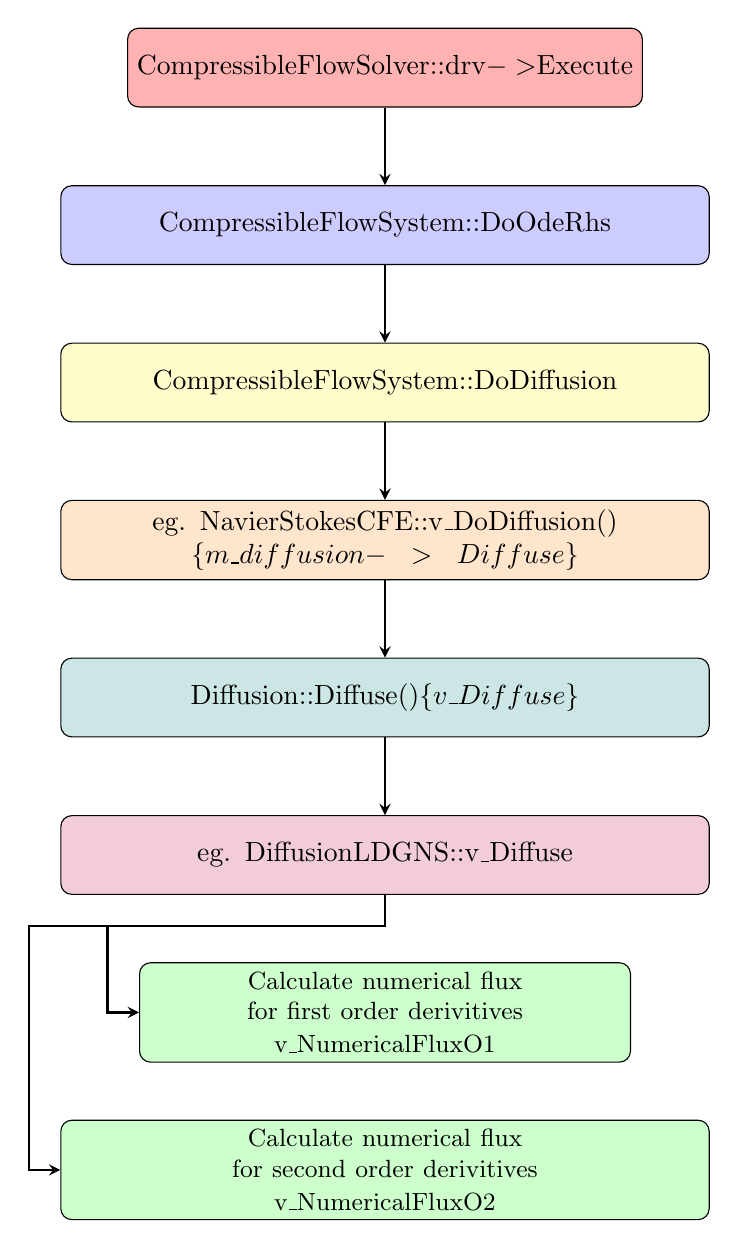
\begin{tikzpicture}[scale=0.2,node distance=2cm]
\node (A)
[rectangle,
rounded corners,
minimum width=3cm,
minimum height=1cm,
text centered,
draw=black,
fill=red!30]
{CompressibleFlowSolver::drv$->$Execute};
\node (B)
[rectangle,
rounded corners,
minimum width=8cm,
minimum height=1cm,
text width=8cm,
text centered,
draw=black,
fill=blue!20,
below of=A,
xshift=0cm,
yshift=0cm]
{CompressibleFlowSystem::DoOdeRhs};
\draw[arrow](A)--(B);
\node (C)
[rectangle,
rounded corners,
minimum width=8cm,
minimum height=1cm,
text width=8cm,
text centered,
draw=black,
fill=yellow!20,
below of=B,
xshift=0cm,
yshift=0cm]
{CompressibleFlowSystem::DoDiffusion};
\draw[arrow](B)--(C);
\node (D)
[rectangle,
rounded corners,
minimum width=8cm,
minimum height=1cm,
text width=8cm,
text centered,
draw=black,
fill=orange!20,
below of=C,
xshift=0cm,
yshift=0cm]
{eg. NavierStokesCFE::v$\_$DoDiffusion()\\$\{m\_diffusion->Diffuse\}$};
\draw[arrow](C)--(D);
\node (E)
[rectangle,
rounded corners,
minimum width=8cm,
minimum height=1cm,
text width=8cm,
text centered,
draw=black,
fill=teal!20,
below of=D,
xshift=0cm,
yshift=0cm]
{Diffusion::Diffuse()$\{v\_Diffuse\}$};
\draw[arrow](D)--(E);
\node (F)
[rectangle,
rounded corners,
minimum width=8cm,
minimum height=1cm,
text width=8cm,
text centered,
draw=black,
fill=purple!20,
below of=E,
xshift=0cm,
yshift=0cm]
{eg. DiffusionLDGNS::v$\_$Diffuse};
\draw[arrow](E)--(F);
\node (G_1)
[rectangle,
rounded corners,
minimum width=6cm,
minimum height=1cm,
text width=6cm,
text centered,
draw=black,
fill=green!20,
below of=F,
xshift=0cm,
yshift=0cm]
{\small{Calculate numerical flux\\ for first order derivitives}\\\small{v$\_$NumericalFluxO1}};
\draw[arrow]($(F.south)$)--++(0,-2cm)-|($(G_1.west)+(-2cm,0)$)--(G_1.west);
% \draw[arrow](E)--(F_1);
\node (G_2)
[rectangle,
rounded corners,
minimum width=8cm,
minimum height=1cm,
text width=8cm,
text centered,
draw=black,
fill=green!20,
below of=G_1,
xshift=0cm,
yshift=0cm]
{\small{Calculate numerical flux\\ for second order derivitives}\\\small{v$\_$NumericalFluxO2}};
\draw[arrow]($(F.south)$)--++(0,-2cm)-|($(G_2.west)+(-2cm,0)$)--(G_2.west);
\end{tikzpicture}
\end{document}